% Options for packages loaded elsewhere
\PassOptionsToPackage{unicode}{hyperref}
\PassOptionsToPackage{hyphens}{url}
\PassOptionsToPackage{dvipsnames,svgnames,x11names}{xcolor}
%
\documentclass[
  letterpaper,
  DIV=11,
  numbers=noendperiod]{scrartcl}

\usepackage{amsmath,amssymb}
\usepackage{iftex}
\ifPDFTeX
  \usepackage[T1]{fontenc}
  \usepackage[utf8]{inputenc}
  \usepackage{textcomp} % provide euro and other symbols
\else % if luatex or xetex
  \usepackage{unicode-math}
  \defaultfontfeatures{Scale=MatchLowercase}
  \defaultfontfeatures[\rmfamily]{Ligatures=TeX,Scale=1}
\fi
\usepackage{lmodern}
\ifPDFTeX\else  
    % xetex/luatex font selection
\fi
% Use upquote if available, for straight quotes in verbatim environments
\IfFileExists{upquote.sty}{\usepackage{upquote}}{}
\IfFileExists{microtype.sty}{% use microtype if available
  \usepackage[]{microtype}
  \UseMicrotypeSet[protrusion]{basicmath} % disable protrusion for tt fonts
}{}
\makeatletter
\@ifundefined{KOMAClassName}{% if non-KOMA class
  \IfFileExists{parskip.sty}{%
    \usepackage{parskip}
  }{% else
    \setlength{\parindent}{0pt}
    \setlength{\parskip}{6pt plus 2pt minus 1pt}}
}{% if KOMA class
  \KOMAoptions{parskip=half}}
\makeatother
\usepackage{xcolor}
\setlength{\emergencystretch}{3em} % prevent overfull lines
\setcounter{secnumdepth}{-\maxdimen} % remove section numbering
% Make \paragraph and \subparagraph free-standing
\ifx\paragraph\undefined\else
  \let\oldparagraph\paragraph
  \renewcommand{\paragraph}[1]{\oldparagraph{#1}\mbox{}}
\fi
\ifx\subparagraph\undefined\else
  \let\oldsubparagraph\subparagraph
  \renewcommand{\subparagraph}[1]{\oldsubparagraph{#1}\mbox{}}
\fi

\usepackage{color}
\usepackage{fancyvrb}
\newcommand{\VerbBar}{|}
\newcommand{\VERB}{\Verb[commandchars=\\\{\}]}
\DefineVerbatimEnvironment{Highlighting}{Verbatim}{commandchars=\\\{\}}
% Add ',fontsize=\small' for more characters per line
\usepackage{framed}
\definecolor{shadecolor}{RGB}{241,243,245}
\newenvironment{Shaded}{\begin{snugshade}}{\end{snugshade}}
\newcommand{\AlertTok}[1]{\textcolor[rgb]{0.68,0.00,0.00}{#1}}
\newcommand{\AnnotationTok}[1]{\textcolor[rgb]{0.37,0.37,0.37}{#1}}
\newcommand{\AttributeTok}[1]{\textcolor[rgb]{0.40,0.45,0.13}{#1}}
\newcommand{\BaseNTok}[1]{\textcolor[rgb]{0.68,0.00,0.00}{#1}}
\newcommand{\BuiltInTok}[1]{\textcolor[rgb]{0.00,0.23,0.31}{#1}}
\newcommand{\CharTok}[1]{\textcolor[rgb]{0.13,0.47,0.30}{#1}}
\newcommand{\CommentTok}[1]{\textcolor[rgb]{0.37,0.37,0.37}{#1}}
\newcommand{\CommentVarTok}[1]{\textcolor[rgb]{0.37,0.37,0.37}{\textit{#1}}}
\newcommand{\ConstantTok}[1]{\textcolor[rgb]{0.56,0.35,0.01}{#1}}
\newcommand{\ControlFlowTok}[1]{\textcolor[rgb]{0.00,0.23,0.31}{#1}}
\newcommand{\DataTypeTok}[1]{\textcolor[rgb]{0.68,0.00,0.00}{#1}}
\newcommand{\DecValTok}[1]{\textcolor[rgb]{0.68,0.00,0.00}{#1}}
\newcommand{\DocumentationTok}[1]{\textcolor[rgb]{0.37,0.37,0.37}{\textit{#1}}}
\newcommand{\ErrorTok}[1]{\textcolor[rgb]{0.68,0.00,0.00}{#1}}
\newcommand{\ExtensionTok}[1]{\textcolor[rgb]{0.00,0.23,0.31}{#1}}
\newcommand{\FloatTok}[1]{\textcolor[rgb]{0.68,0.00,0.00}{#1}}
\newcommand{\FunctionTok}[1]{\textcolor[rgb]{0.28,0.35,0.67}{#1}}
\newcommand{\ImportTok}[1]{\textcolor[rgb]{0.00,0.46,0.62}{#1}}
\newcommand{\InformationTok}[1]{\textcolor[rgb]{0.37,0.37,0.37}{#1}}
\newcommand{\KeywordTok}[1]{\textcolor[rgb]{0.00,0.23,0.31}{#1}}
\newcommand{\NormalTok}[1]{\textcolor[rgb]{0.00,0.23,0.31}{#1}}
\newcommand{\OperatorTok}[1]{\textcolor[rgb]{0.37,0.37,0.37}{#1}}
\newcommand{\OtherTok}[1]{\textcolor[rgb]{0.00,0.23,0.31}{#1}}
\newcommand{\PreprocessorTok}[1]{\textcolor[rgb]{0.68,0.00,0.00}{#1}}
\newcommand{\RegionMarkerTok}[1]{\textcolor[rgb]{0.00,0.23,0.31}{#1}}
\newcommand{\SpecialCharTok}[1]{\textcolor[rgb]{0.37,0.37,0.37}{#1}}
\newcommand{\SpecialStringTok}[1]{\textcolor[rgb]{0.13,0.47,0.30}{#1}}
\newcommand{\StringTok}[1]{\textcolor[rgb]{0.13,0.47,0.30}{#1}}
\newcommand{\VariableTok}[1]{\textcolor[rgb]{0.07,0.07,0.07}{#1}}
\newcommand{\VerbatimStringTok}[1]{\textcolor[rgb]{0.13,0.47,0.30}{#1}}
\newcommand{\WarningTok}[1]{\textcolor[rgb]{0.37,0.37,0.37}{\textit{#1}}}

\providecommand{\tightlist}{%
  \setlength{\itemsep}{0pt}\setlength{\parskip}{0pt}}\usepackage{longtable,booktabs,array}
\usepackage{calc} % for calculating minipage widths
% Correct order of tables after \paragraph or \subparagraph
\usepackage{etoolbox}
\makeatletter
\patchcmd\longtable{\par}{\if@noskipsec\mbox{}\fi\par}{}{}
\makeatother
% Allow footnotes in longtable head/foot
\IfFileExists{footnotehyper.sty}{\usepackage{footnotehyper}}{\usepackage{footnote}}
\makesavenoteenv{longtable}
\usepackage{graphicx}
\makeatletter
\def\maxwidth{\ifdim\Gin@nat@width>\linewidth\linewidth\else\Gin@nat@width\fi}
\def\maxheight{\ifdim\Gin@nat@height>\textheight\textheight\else\Gin@nat@height\fi}
\makeatother
% Scale images if necessary, so that they will not overflow the page
% margins by default, and it is still possible to overwrite the defaults
% using explicit options in \includegraphics[width, height, ...]{}
\setkeys{Gin}{width=\maxwidth,height=\maxheight,keepaspectratio}
% Set default figure placement to htbp
\makeatletter
\def\fps@figure{htbp}
\makeatother

<link href="bayesian_final_project_files/libs/htmltools-fill-0.5.8.1/fill.css" rel="stylesheet" />
<script src="bayesian_final_project_files/libs/htmlwidgets-1.6.4/htmlwidgets.js"></script>
<script src="bayesian_final_project_files/libs/viz-1.8.2/viz.js"></script>
<link href="bayesian_final_project_files/libs/DiagrammeR-styles-0.2/styles.css" rel="stylesheet" />
<script src="bayesian_final_project_files/libs/grViz-binding-1.0.11/grViz.js"></script>
\KOMAoption{captions}{tableheading}
\makeatletter
\@ifpackageloaded{tcolorbox}{}{\usepackage[skins,breakable]{tcolorbox}}
\@ifpackageloaded{fontawesome5}{}{\usepackage{fontawesome5}}
\definecolor{quarto-callout-color}{HTML}{909090}
\definecolor{quarto-callout-note-color}{HTML}{0758E5}
\definecolor{quarto-callout-important-color}{HTML}{CC1914}
\definecolor{quarto-callout-warning-color}{HTML}{EB9113}
\definecolor{quarto-callout-tip-color}{HTML}{00A047}
\definecolor{quarto-callout-caution-color}{HTML}{FC5300}
\definecolor{quarto-callout-color-frame}{HTML}{acacac}
\definecolor{quarto-callout-note-color-frame}{HTML}{4582ec}
\definecolor{quarto-callout-important-color-frame}{HTML}{d9534f}
\definecolor{quarto-callout-warning-color-frame}{HTML}{f0ad4e}
\definecolor{quarto-callout-tip-color-frame}{HTML}{02b875}
\definecolor{quarto-callout-caution-color-frame}{HTML}{fd7e14}
\makeatother
\makeatletter
\makeatother
\makeatletter
\makeatother
\makeatletter
\@ifpackageloaded{caption}{}{\usepackage{caption}}
\AtBeginDocument{%
\ifdefined\contentsname
  \renewcommand*\contentsname{Table of contents}
\else
  \newcommand\contentsname{Table of contents}
\fi
\ifdefined\listfigurename
  \renewcommand*\listfigurename{List of Figures}
\else
  \newcommand\listfigurename{List of Figures}
\fi
\ifdefined\listtablename
  \renewcommand*\listtablename{List of Tables}
\else
  \newcommand\listtablename{List of Tables}
\fi
\ifdefined\figurename
  \renewcommand*\figurename{Figure}
\else
  \newcommand\figurename{Figure}
\fi
\ifdefined\tablename
  \renewcommand*\tablename{Table}
\else
  \newcommand\tablename{Table}
\fi
}
\@ifpackageloaded{float}{}{\usepackage{float}}
\floatstyle{ruled}
\@ifundefined{c@chapter}{\newfloat{codelisting}{h}{lop}}{\newfloat{codelisting}{h}{lop}[chapter]}
\floatname{codelisting}{Listing}
\newcommand*\listoflistings{\listof{codelisting}{List of Listings}}
\makeatother
\makeatletter
\@ifpackageloaded{caption}{}{\usepackage{caption}}
\@ifpackageloaded{subcaption}{}{\usepackage{subcaption}}
\makeatother
\makeatletter
\@ifpackageloaded{tcolorbox}{}{\usepackage[skins,breakable]{tcolorbox}}
\makeatother
\makeatletter
\@ifundefined{shadecolor}{\definecolor{shadecolor}{rgb}{.97, .97, .97}}
\makeatother
\makeatletter
\makeatother
\makeatletter
\makeatother
\ifLuaTeX
  \usepackage{selnolig}  % disable illegal ligatures
\fi
\IfFileExists{bookmark.sty}{\usepackage{bookmark}}{\usepackage{hyperref}}
\IfFileExists{xurl.sty}{\usepackage{xurl}}{} % add URL line breaks if available
\urlstyle{same} % disable monospaced font for URLs
\hypersetup{
  pdftitle={Bayesian Model Course Final Project},
  pdfauthor={Maria Adelia Widijanto},
  colorlinks=true,
  linkcolor={blue},
  filecolor={Maroon},
  citecolor={Blue},
  urlcolor={Blue},
  pdfcreator={LaTeX via pandoc}}

\title{Bayesian Model Course Final Project}
\author{Maria Adelia Widijanto}
\date{}

\begin{document}
\maketitle
\ifdefined\Shaded\renewenvironment{Shaded}{\begin{tcolorbox}[enhanced, borderline west={3pt}{0pt}{shadecolor}, interior hidden, breakable, frame hidden, boxrule=0pt, sharp corners]}{\end{tcolorbox}}\fi

\hypertarget{introduction}{%
\section{Introduction}\label{introduction}}

This document outlines the Bayesian framework described in \textbf{Levy
et al.~(2018), ``Estimation of Gross Land-Use Change and Its Uncertainty
Using a Bayesian Data Assimilation Approach'' (Biogeosciences, 15(5),
1497-1513).} The paper introduces a novel approach for estimating
land-use change by addressing the challenge posed by multiple sources of
land-use maps of an area. By employing a Bayesian framework, these
diverse sources are treated as prior information, which is then
assimilated to generate a more refined and cohesive land-use map.

The Bayesian framework was applied to what the author was referring to
\textbf{data assimilation}, which defines as ``an approach for fusing
observations with prior knowledge (e.g.~mathematical representations of
physical laws; model output) to obtain an estimate of the distribution
of the true state of some phenomenon''. In this case, the data
assimilation process corresponds with the prior and likelihood
development process for the Bayesian framework.

\hypertarget{research-question}{%
\subsection{Research Question}\label{research-question}}

\begin{description}
\item[The research question of this paper is]
How can a Bayesian hierarchical model be developed and applied to
integrate multiple data sources to produce accurate and spatially
explicit estimates of land-use change over time?
\end{description}

In a case study, they applied the approach to Scotland over the period
1969-2015

\hypertarget{model-description}{%
\section{Model Description}\label{model-description}}

\hypertarget{data-structure}{%
\subsection{Data Structure}\label{data-structure}}

We begin with historical land use maps, denoted as \(\mathbf{U}\), which
represent land use types at each grid location on the map. Each grid
location is specified by coordinates \(x\) and \(y\), making
\(\mathbf{U_{xy}}\) a vector that describes land use at a particular
location. By utilizing maps from multiple time points, we can construct
a land use transition matrix, \(\mathbf{B}\), for each time step \(t\).

The land use transition matrix \(\mathbf{B}\) is defined as:

\[
B = 
\begin{bmatrix}
0 & \beta_{12} & \beta_{13} & \dots & \beta_{1n} \\
\beta_{21} & 0 & \beta_{23} & \dots & \beta_{2n} \\
\vdots & \vdots & \vdots & \ddots & \vdots \\
\beta_{n1} & \beta_{n2} & \beta_{n3} & \dots & 0
\end{bmatrix}
\quad t=1
\]

This continues for each time step \(t\):

\[
\vdots
\]

\[
\begin{bmatrix}
0 & \beta_{12} & \beta_{13} & \dots & \beta_{1n} \\
\beta_{21} & 0 & \beta_{23} & \dots & \beta_{2n} \\
\vdots & \vdots & \vdots & \ddots & \vdots \\
\beta_{n1} & \beta_{n2} & \beta_{n3} & \dots & 0
\end{bmatrix}
\quad t=n_t
\]

where each \(\beta_{ij}\) element represents the area of land use class
\(i\) (rows) that transitioned to class \(j\) (columns) at time step
\(t\), measured in square kilometers (km\textsuperscript{2}).

To calculate \(\beta_{ijt}\), we use data from \(\mathbf{U_{xy}}\):

\[
\beta_{ijt} = \sum_{x=1}^{n_x} \sum_{y=1}^{n_y} \left[ U_{xyt-1} = i \land U_{xyt} = j \right] l^2 \tag{3}
\]

where \(l\) denotes the grid size of the map. By knowing these
variables, we can express the net change in land use \(\Delta A_{ut}\)
using the net area difference:

\[
\Delta A_{ut} = A_{ut} - A_{ut-1} \tag{2}
\]

Alternatively, we can calculate \(\Delta A_{ut}\) using the transition
matrix \(\mathbf{B}\) by determining the gross gains (column sum vector,
\(\mathbf{G_t}\)) and the gross losses (row sum vector,
\(\mathbf{L_t}\)):

\[
\Delta A_{ut} = G_{ut} - L_{ut} \tag{4}
\]

where

\[
G_{ut} = \sum_{i=1}^{n_u} \beta_{iut}
\]

and

\[
L_{ut} = \sum_{j=1}^{n_u} \beta_{ujt}
\]

Knowing the parameters of \(\mathbf{U}\), \(\mathbf{B}\), and
\(\mathbf{A}\), the author did two step of methods:

\begin{enumerate}
\def\labelenumi{\arabic{enumi}.}
\item
  The author first applied the \textbf{Bayesian approach} to estimate
  the parameters in \(\mathbf{B}\). In this framework, we specify prior
  information about \(\mathbf{B}\) and use the likelihood based on
  partial observations of \(\mathbf{U}\) and \(\mathbf{A}\). This
  results in a posterior distribution for \(\mathbf{B}\).
\item
  The authors then use this posterior distribution of \(\mathbf{B}\)
  along with a probability weighting matrix \(\mathbf{W}\) to conduct a
  \textbf{weighted sampling operation}. This process simulates where
  land-use changes are likely to occur, generating posterior
  realizations of \(\mathbf{U}\).
\end{enumerate}

\hypertarget{estimating-posterior-distribution-of-transtition-matrix}{%
\subsection{Estimating posterior distribution of transtition
matrix}\label{estimating-posterior-distribution-of-transtition-matrix}}

\hypertarget{the-priors}{%
\subsubsection{The Priors}\label{the-priors}}

The priors are derived from data provided by the Countryside Survey
(CS), which offers direct observations of \(\mathbf{B}\) over multiple
years. This results in a matrix of \(\mathbf{B^{prior}}\).

\hypertarget{the-observations}{%
\subsubsection{The Observations}\label{the-observations}}

\begin{enumerate}
\def\labelenumi{\arabic{enumi}.}
\item
  The Agricultural Census (AC) provided the total area in the
  agricultural land use, which is one out of six land use category being
  analyzed in this paper. This data is then can be used as the
  \(\mathbf{A_{ut}^{obs}}\) . By using the information from
  \(\mathbf{B^{prior}}\) into \(Eq. 4\) and combining different \(t\)
  observation years, \(\Delta \mathbf{A_{ut}^{obs}}\) could be gained.
\item
  The EDINA Agricultural Census (EAC) provided the detailed information
  of the \(\mathbf{L_t}\) and \(\mathbf{G_t}\).
\item
  Using Corine, IACS, and FC maps, \(\mathbf{U^{obs}}\) matrices are
  gained and used as an input for \(Eq. 3\), which resulted in
  \(\mathbf{B_{t}^{obs}}\) as the observed transition matrix for each
  year.
\end{enumerate}

\hypertarget{the-likelihoods}{%
\subsubsection{The Likelihoods}\label{the-likelihoods}}

These multiple data sets were being used by the author to develop each
of the likelihood based on the each observation variables.

\begin{enumerate}
\def\labelenumi{\arabic{enumi}.}
\tightlist
\item
  Using the \(\Delta \mathbf{A_{ut}^{obs}}\) information,
  \(\mathcal{L_{net}}\) was established, which is the likelihood based
  on the overall area change that follows a normal distribution:
\end{enumerate}

\[\mathcal{L}_{net} = \prod_{u=1}^{n_u} \prod_{t=1}^{n_t} \frac{1}{\sigma_{ut}\sqrt{2\pi}} \exp \left( -\frac{(\Delta A_{ut}^{obs} - \Delta A_{ut}^{pred})^2}{2 \sigma_{ut}^2} \right) \tag{5}\]

with \(\sigma_{ut}\) being the observational error of the data.

\begin{enumerate}
\def\labelenumi{\arabic{enumi}.}
\setcounter{enumi}{1}
\tightlist
\item
  Using the \(\mathbf{G}\) and \(\mathbf{L}\), the likelihood of the
  gross area change (\(\mathcal{L_{gross}})\) can be calculated, however
  because of the nature of the data, the likelihood distribution is
  corrected using a skew parameter, making this a skewed normal
  distribution
\end{enumerate}

\[\mathcal{L}_{gross} = \prod_{u=1}^{n_u} \prod_{t=1}^{n_t} \frac{2}{\sigma_{L_{ut}}^{obs}} \phi \left( \frac{L_{ut}^{obs} - L_{ut}^{pred}}{\sigma_{L_{ut}}^{obs}} \right) 
\Phi \left( \alpha \frac{L_{ut}^{obs} - L_{ut}^{pred}}{\sigma_{L_{ut}}^{obs}} \right) 
\times \frac{2}{\sigma_{G_{ut}}^{obs}} 
\phi \left( \frac{G_{ut}^{obs} - G_{ut}^{pred}}{\sigma_{G_{ut}}^{obs}} \right) 
\Phi \left( \alpha \frac{G_{ut}^{obs} - G_{ut}^{pred}}{\sigma_{G_{ut}}^{obs}} \right) \tag{6}\]

where \(\phi\) is the standard normal probability density function,
\(\Phi\) is the corresponding cumulative density function, and
\(\alpha\) is the skew parameter.

\begin{enumerate}
\def\labelenumi{\arabic{enumi}.}
\setcounter{enumi}{2}
\tightlist
\item
  Using \(\mathbf{B_{t}^{obs}}\), a likelihood of the predicted
  transition matrix (\(\mathcal{L}_{B}\)) can be calculated as follow:
\end{enumerate}

\[
\mathcal{L}_{B} = \prod_{i=1}^{n_u} \prod_{j=1}^{n_i} \prod_{t=1}^{n_t} \frac{1}{\sigma_{\beta_{ijt}}^{\text{obs}} \sqrt{2\pi}} \exp \left( -\frac{\left( \beta_{ijt}^{\text{obs}} - \beta_{ijt}^{\text{pred}} \right)^2}{2 \left( \sigma_{\beta_{ijt}}^{\text{obs}} \right)^2} \right) \tag{7}
\]

\hypertarget{jags-model}{%
\subsubsection{JAGS model}\label{jags-model}}

While the authors did not provide any specific code to show the analysis
process, they mentioned that they used \texttt{BayesianTools} package
instead of running it on \texttt{rjags}. Nevertheless, the simplified
\texttt{rjags} model framework would look something like this:

\begin{Shaded}
\begin{Highlighting}[]
\NormalTok{model\_dummy }\OtherTok{\textless{}{-}} \StringTok{"}
\StringTok{model\{}
\StringTok{  }
\StringTok{\#\#\# PRIORS \#\#\#}

\StringTok{\# B\_prior represents prior B matrix about land use transitions from the CS data.}
\StringTok{for (i in 1:n\_u) \{ \# n\_u is the total number of land use classes}
\StringTok{  for (j in 1:n\_t) \{ \#n\_t is the number of timesteps}
\StringTok{    B[i, j] \textasciitilde{} dnorm(B\_prior[i, j], tau\_B) \# tau\_B is the precision (inverse of variance) of the prior distribution (sigma\_B\^{}2)}
\StringTok{\# sigma\_B was calculated using bootstraping approach}
\StringTok{  \}}
\StringTok{\}}

\StringTok{\# Prior for observational error}

\StringTok{\# Assuming that the standard deviations are between x1 and x2 which the author did not specifically defined (will be explained in the next part)}
\StringTok{\# sigma\_A, sigma\_L, and sigma\_G represent the standard deviation for the observational errors.}
\StringTok{sigma\_A \textasciitilde{} dunif(x1, x2)  }
\StringTok{sigma\_L \textasciitilde{} dunif(x1, x2)  }
\StringTok{sigma\_G \textasciitilde{} dunif(x1, x2)}

\StringTok{\# each sigma will be used to calculate each tau with tau = 1/sigma\^{}2}
\StringTok{tau\_A \textless{}{-} 1/sigma\_A}
\StringTok{tau\_L \textless{}{-} 1/sigma\_L}
\StringTok{tau\_G \textless{}{-} 1/sigma\_G}

\StringTok{\#\#\# LIKELIHOOD \#\#\#}

\StringTok{\# Likelihood for L\_net (overall area change)}
\StringTok{\# delta\_A\_obs\_ follows a normal distribution centered at ΔA\_pred\_ut with variance based on sigma\_A.}
\StringTok{for (u in 1:n\_u) \{}
\StringTok{  for (t in 1:n\_t) \{}
\StringTok{    delta\_A\_obs[u, t] \textasciitilde{} dnorm(delta\_A\_pred[u, t], tau\_A)}

\StringTok{  \}}
\StringTok{\}}

\StringTok{\# Likelihood for L\_gross (gross area change) with skewed normal distribution}
\StringTok{\# L\_obs\_ut and G\_obs\_ut follow skewed distributions based on parameters sigma\_L, sigma\_G, and skew parameter alpha.}
\StringTok{for (u in 1:n\_u) \{}
\StringTok{  for (t in 1:n\_t) \{}
\StringTok{    L\_obs[u, t] \textasciitilde{} dsnorm(L\_pred[u, t], tau\_L, alpha\_L)}
\StringTok{    G\_obs[u, t] \textasciitilde{} dsnorm(G\_pred[u, t], tau\_G, alpha\_G)}
\StringTok{  \}}
\StringTok{\}}
\StringTok{\# alpha\_L and alpha\_G are skewness parameters.}

\StringTok{\# Likelihood for L\_B (predicted transition matrix)}
\StringTok{\# beta\_obs\_ijt follows a normal distribution centered at beta\_pred\_ijt with variance based on sigma\_B.}
\StringTok{for (i in 1:n\_i) \{ \# n\_i is the t{-}1 land use class}
\StringTok{  for (j in 1:n\_j) \{ \# n\_t is the t land use class}
\StringTok{    for (t in 1:n\_t) \{ \# n\_t is the time step}
\StringTok{      beta\_obs[i, j, t] \textasciitilde{} dnorm(beta\_pred[i, j, t], tau\_B)}
\StringTok{    \}}
\StringTok{  \}}
\StringTok{\}}

\StringTok{\# Unelaborated overall likelihood: summation of each log likelihoods}
\StringTok{\}}
\StringTok{  \}}
\StringTok{\} "}
\end{Highlighting}
\end{Shaded}

The overall likelihood is a sum of the log of each of the likelihoods
(equation not elaborated).

After defining model, we could then continue to fit the model. To
simplify the process, the observed data could be a list object that
stores the map information (possibly turn them first into matrix
format). This list object is named \texttt{data\_input} in this example.
The information given in the text article is that \emph{``nine chains
were used, with 100 000 iterations in each. To establish the initial}
\(B\) \emph{parameter values for one of the chains, a least-squares fit
with the} \(\Delta{A}\) \emph{was used. Other chains were over dispersed
by adding random variation to this best-fit parameter set.''}.

Since we have a specific initial values for B, we could define it
specifically. But to keep things simple, as the same concept with the
inputs, the initial values of the iterations can be defined as stored as
a list object which in this case is called \texttt{inits\_list}.

\begin{Shaded}
\begin{Highlighting}[]
\FunctionTok{library}\NormalTok{(rjags)}
\NormalTok{model }\OtherTok{\textless{}{-}} \FunctionTok{jags.model}\NormalTok{(}\FunctionTok{textConnection}\NormalTok{(model\_dummy), }
                    \CommentTok{\#data = data\_input, }
                    \CommentTok{\#inits = inits\_list, }
                    \AttributeTok{n.chains =} \DecValTok{9}
\NormalTok{                    )}
\end{Highlighting}
\end{Shaded}

\begin{verbatim}
Error in jags.model(textConnection(model_dummy), n.chains = 9): 
Error parsing model file:
syntax error on line 60 near "}"
\end{verbatim}

We then apply the MCMC sampling to the model with 100 000 to establish
the posterior distribution of \(B^{post}\)

\begin{Shaded}
\begin{Highlighting}[]
\NormalTok{samples }\OtherTok{\textless{}{-}} \FunctionTok{coda.samples}\NormalTok{(model, }
                        \AttributeTok{variable.names =} \FunctionTok{c}\NormalTok{(}\StringTok{"B\_post"}\NormalTok{), }
                        \AttributeTok{n.iter =} \DecValTok{100000}\NormalTok{)}
\end{Highlighting}
\end{Shaded}

\begin{verbatim}
Error: object 'model' not found
\end{verbatim}

\begin{tcolorbox}[enhanced jigsaw, toprule=.15mm, arc=.35mm, bottomtitle=1mm, colframe=quarto-callout-note-color-frame, coltitle=black, rightrule=.15mm, leftrule=.75mm, titlerule=0mm, opacitybacktitle=0.6, bottomrule=.15mm, colback=white, toptitle=1mm, title=\textcolor{quarto-callout-note-color}{\faInfo}\hspace{0.5em}{Why did the author chose this parameters to run the MCMC?}, breakable, left=2mm, opacityback=0, colbacktitle=quarto-callout-note-color!10!white]

Note that there are five types of callouts, including: \texttt{note},
\texttt{warning}, \texttt{important}, \texttt{tip}, and
\texttt{caution}.

\end{tcolorbox}

\hypertarget{estimating-updated-land-cover-with-the-new-transition-matrix}{%
\subsection{Estimating Updated Land Cover with the New Transition
Matrix}\label{estimating-updated-land-cover-with-the-new-transition-matrix}}

After obtaining \(\mathbf{B^{post}}\), the authors had the information
of each land use change area allocation from class \(i\) to \(j\) for
each time step \(t\) . Using this information, then used the
\(\mathbf{U^{obs}}\) from \(t\) and \(t-1\) to allocate cell grids that
are being sampled for each transition from \(i\) to \(j\). The rule of
the sampling is represented as follow:

\[
\begin{align*}    W_{xy} &\leftarrow     \begin{cases}        0, & \text{if } U_{xy,t}^{obs} \neq i \\        1, & \text{else}    \end{cases}    \\    W_{xy} &\leftarrow     \begin{cases}        1, & \text{if } U_{xy,t-1}^{obs} = j \\        p_m, & \text{else}    \end{cases}\end{align*}
\]

with \(p_{m}\) being the probability of cells being misclassified in
\(U^{obs}\) .

\begin{tcolorbox}[enhanced jigsaw, toprule=.15mm, arc=.35mm, bottomtitle=1mm, colframe=quarto-callout-tip-color-frame, coltitle=black, rightrule=.15mm, leftrule=.75mm, titlerule=0mm, opacitybacktitle=0.6, bottomrule=.15mm, colback=white, toptitle=1mm, title=\textcolor{quarto-callout-tip-color}{\faLightbulb}\hspace{0.5em}{Example of weighted sampling operation}, breakable, left=2mm, opacityback=0, colbacktitle=quarto-callout-tip-color!10!white]

It is known from the \(\mathbf{B^{post}}\) that seven grid cells change
from grass to crop from 2014 to 2015. The model selects candidate cells
that are crop in 2015, with a higher probability given to the same cells
that were grass in 2014. If the posterior estimate
\(\beta_{ijt}^{post}\) (the predicted area of change from crop to grass)
is smaller than the observed value \(\beta_{ijt}^{obs}\), only a subset
of the high-probability cells will be selected. The process results in
the number of cells that most likely to change are those identified as
crops in 2015 and as grass in 2014, based on the weighting criteria
\(\mathbf{W}\).

\end{tcolorbox}

The method to conduct weighted sampling is not elaborated in this
report, but could be done in R with different packages available.

\hypertarget{directed-acyclic-graphs-dag}{%
\subsection{Directed Acyclic Graphs
(DAG)}\label{directed-acyclic-graphs-dag}}

The simplified structure of this Bayesian application can be visualized
as follow

\hypertarget{results}{%
\section{Results}\label{results}}

\textbf{MCMC result:} Although not shown, the authors ran several
convergence diagnostics and mentioned that the MCMC converged, providing
a reasonable estimate of the posterior distribution of B.

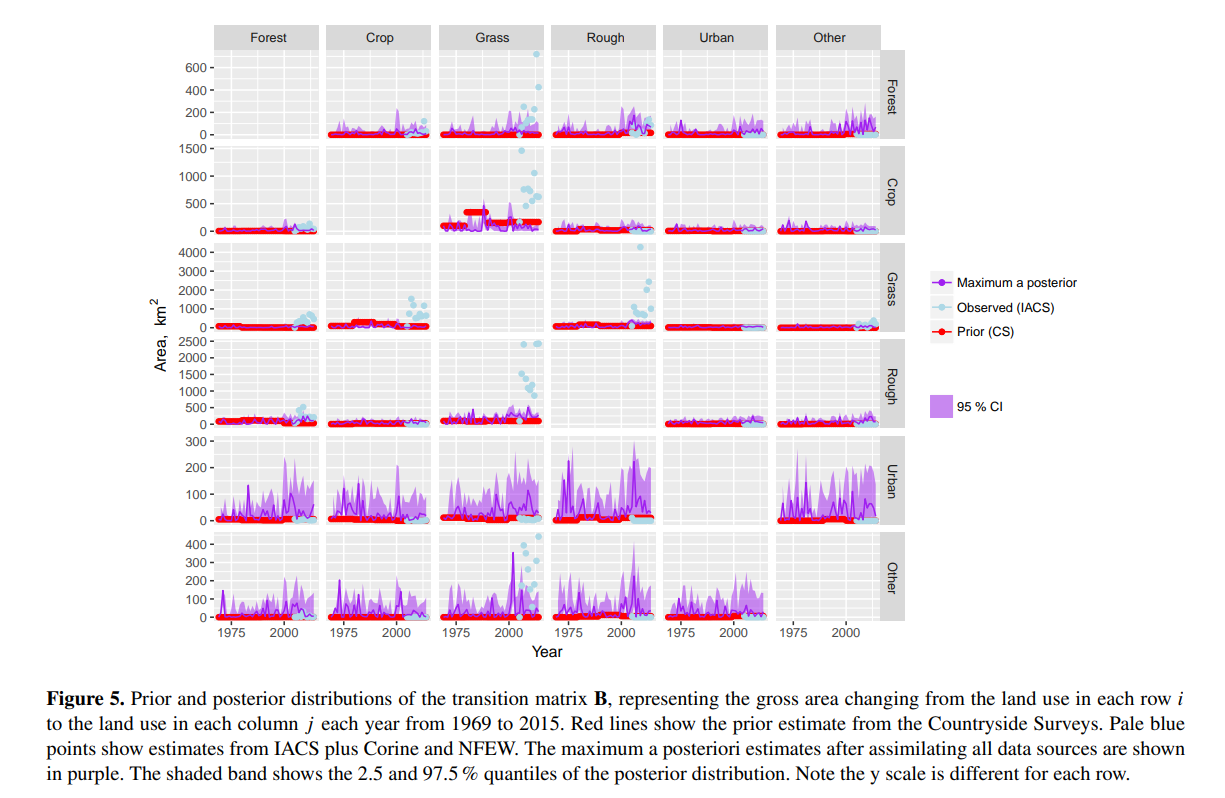
\includegraphics{bayesian_final_project_files/figures/fig_5.png} Figure
5 reveals diverse patterns in how the posterior distribution results
differ across changes in \(\beta_{ij}\), compared with the prior
distribution. \textbf{These significant differences suggest that the
model learned considerably from the data, while minimal differences
indicate a stronger reliance on prior information.}

\subsubsection{Gains}

\begin{figure}

{\centering 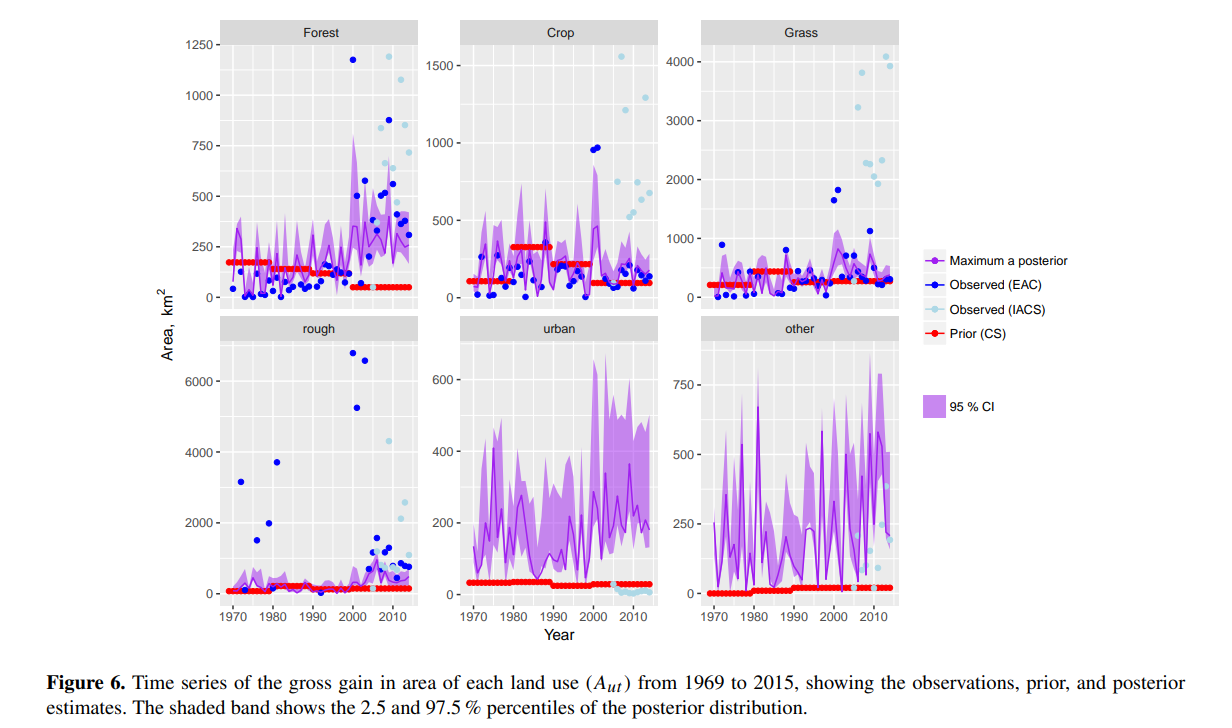
\includegraphics{bayesian_final_project_files/figures/fig_6.png}

}

\caption{Fig. 6: Gains}

\end{figure}

\subsubsection{Loss}

\begin{figure}

{\centering 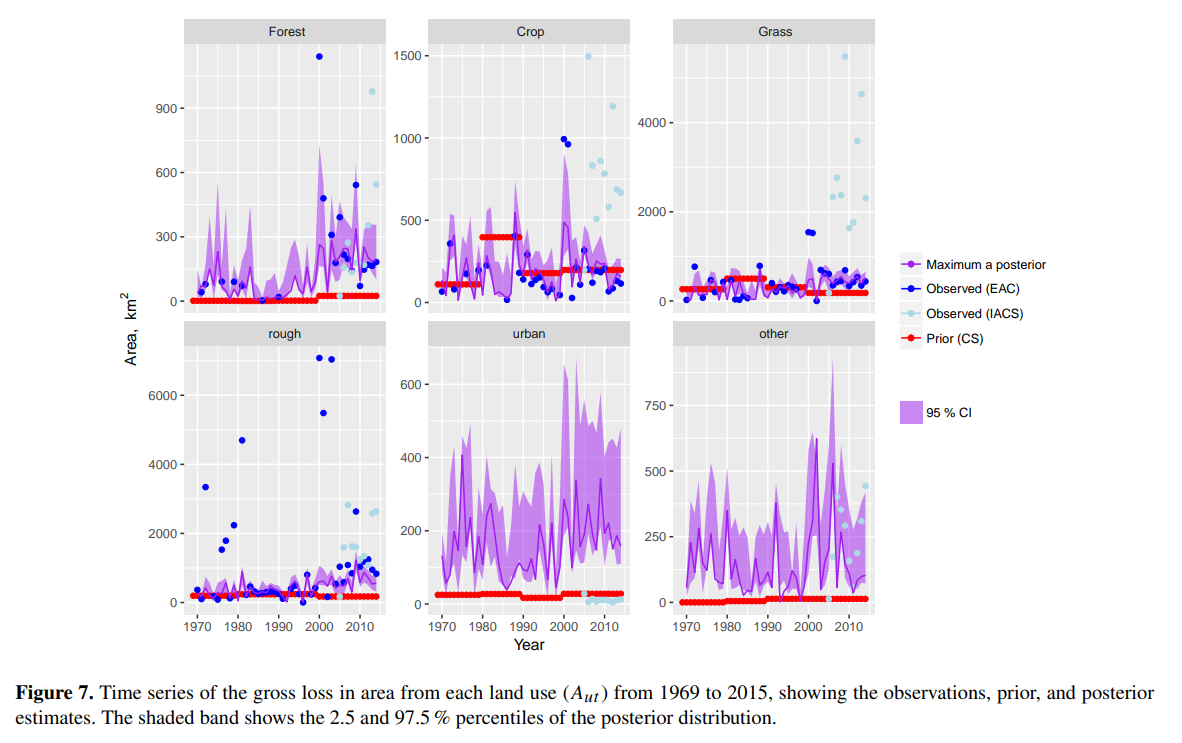
\includegraphics{bayesian_final_project_files/figures/fig_7.png}

}

\caption{Fig. 7: Loss}

\end{figure}

Figures 6 and 7 show the total area gained and lost for each land use.
The same observations can be inferred as in Figure 5, where each class
has its own variability. One factor that can explain these variations
between classes is the difference in how each observation dataset
categorizes land use classes. For example, there are fewer observation
data for urban and other land-use areas, which results in less
constraint on the posterior. The authors also raised this as a potential
issue, mentioning that harmonizing land use classifications from
different datasets ``may not be comparing to like to like''.



\end{document}
